\title{Cost of language Java}
\author{
        Martin Kozeny\\
        CSCI 4501: Programming Language Structure\\
        Spring 2011
        University of New Orleans
}
\date{\today}




\documentclass[5pt]{article}
\usepackage{graphicx}

\setlength{\hoffset}{-2.3cm} 
\setlength{\voffset}{-3cm}
\setlength{\textheight}{24.0cm} 
\setlength{\textwidth}{16cm}


\begin{document}


\maketitle


\paragraph{Programmer training - 4/10}
Java is non-orthogonal and multiplicity language. Multipicity means, that there
is more than one way to express something; e.g. different ways to express loop
(for cycle, while \ldots), different ways to increment (
\verb|count = count+1; count += 1; count++; ++count| ). Non-orthogonal means,
that operations have side effects (e.g. iteration over collection has side
effect - when removing something from collection you skip an element).


\begin{verbatim}
for(int i=0; i<collection.size(); i++)
{
    if(something)
        collection.remove(i);
}\end{verbatim}


It is a function of Simplicity and Orthogonality, so train a Java programmer is
very hard.

\paragraph{Program writing (program development) - 6/10}
It is also connected with Simplicity and Orthogonality. Close to naturalness of
its expression. Data abstraction - Integers are abstracted into class. Lot of
primitives. Programmer does not have to care about memory allocation and other
low level stuff.

\paragraph{Program translation (compilation, interpretation) - 7/10}
Better portability ( than e.g. other high-level language C++) - do not have to
recompile for other types of machines. Price we pay for it is slower execution
( see figure \ref{fig:translation} ).

\begin{figure}[ht]
  \centering
  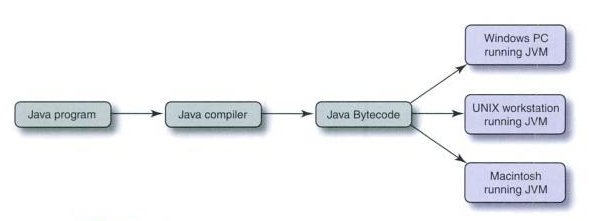
\includegraphics[height=1.35in,width=3.6in]{img/program_translation}
  \caption{Program translation}
  \label{fig:translation}
\end{figure}



\paragraph{Program execution - 6/10}
Because of interpreting, Java is slower than languages, which are compiled.
Downcasting due to polymorphism, creating method table and partly dynamic type
checking due to single dispatch - all is done during run-time and makes
execution slower ( see figure \ref{fig:execution} ).

\begin{figure}[ht]
  \centering
  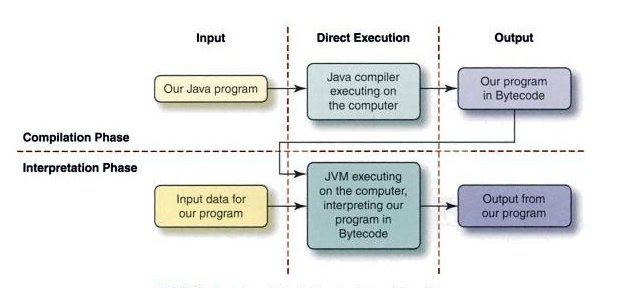
\includegraphics[height=1.64in,width=3.6in]{img/program_execution}
  \caption{Program execution}
  \label{fig:execution}
\end{figure}

\paragraph{Language implementation system - 10/10}
Main reason for rapid application of Java. For eneterprise applications there is
Java EE ( Java2EE = enterprise edition ) used in many application frameworks (
Seam, JSF, \ldots ). For creating applets, desktop applications is appropriate
Java SE ( standard edition ) and for mobile applications Java ME ( mobile
edition ).

\paragraph{Program Reliability - 8/10}
Type checking during compile time and also during run-time. Subscript ranges are
also checked. In Java exists exception handling. Programmer can never have a
dangling pointer but memory leaks can exist. Also there is a problem, that int
can be used as parameter to the function where float is expected.

\paragraph{Program safety and Security - 9/10}
To enforce safety, program in Java is prevented from accessing memory in
inappropriate way. Every piece of memory is a part of Java object. Type safety:
program cannot perfom operation on an object, unless that operation is valid for that
object. Java support dynamic type checking, but if it is possible it is better
to use static type checking.Type safety guarantees that programs will not do
terrible and dangerous things such as treating pointers as integers or falling
off the end of an array ( problem in C++ but not in Java ).

\paragraph{Program maintenance - 8/10}
Correction and modification can be done easily due to inheritance. Static typing
is also useful during maintenance ( you know what returns concrete funtion ).
Java support massive class library. On the other hand Java is non-orthogonal and multiplicity languge which results in poor readability and poor maintenace.










\end{document}
